\documentclass[fontsize=11pt]{scrartcl}
\usepackage[utf8]{inputenc}
\usepackage{color}
\usepackage{hyperref}
\usepackage{graphicx}



\title{Research Notes NASA Ames Joerg Dec18--Jan19}
\author{J\"org Hoffmann, Jeremy Frank, Minh Do, ... }
\date{December 2018}

%%%%%%%%%%% comments %%%%%%%%%%%%

\newcommand{\joerg}[1]{\textcolor{green}{JOERG: \textbf{#1}}}
\newcommand{\jeremy}[1]{\textcolor{green}{JEREMY: \textbf{#1}}}
\renewcommand{\j}[1]{\textcolor{green}{J: \textbf{#1}}}
\newcommand{\minh}[1]{\textcolor{green}{MINH: \textbf{#1}}}
\newcommand{\dave}[1]{\textcolor{green}{DAVE: \textbf{#1}}}

\newcommand{\cool}[1]{\textcolor{blue}{COOL: \textbf{#1}}}

\newcommand{\new}[1]{\textcolor{red}{NEW: \textbf{#1}}}


%%%%%%%%%%% general %%%%%%%%%%%%

\newtheorem{corollary}{Corollary}
\newtheorem{lemma}{Lemma}
\newtheorem{theorem}{Theorem}
\newtheorem{definition}{Definition}
\newtheorem{proposition}{Proposition}
\newtheorem{example}{Example}
\usepackage{placeins}

\newcommand{\defined}[1]{\emph{#1}}

%%%%%%%%%%% heuristics %%%%%%%%%%%%

\newcommand{\hrefine}{\ensuremath{h_{r}}}
\newcommand{\hboth}{\ensuremath{h_{r+b}}}
\newcommand{\hbellman}{\ensuremath{h_{b}}}

\newcommand{\abs}{\mathcal{A}}
\newcommand{\numtasks}[1]{\tiny{(#1)}}

%\newcommand{\formalspacesave}{}

\newcommand{\ie}{i.\,e.}
\newcommand{\eg}{e.\,g.}
\newcommand{\cf}{cf.}
\newcommand{\naturals}{\ensuremath{\mathbb N}}
\newcommand{\reals}{{\mathbb{R}}}
\newcommand{\powerset}{{\mathcal{P}}}

\newcommand{\tuple}[1]{\ensuremath{\langle #1 \rangle}}

\newcommand{\astar}{\ensuremath{\textrm{A}^*}}

\newcommand{\poly}{\textbf{P}}
\newcommand{\np}{\textbf{NP}}
\newcommand{\pspace}{\textbf{PSPACE}}


%%%%%%%%%%%%%%%%%%%%%%%%%%%%%%
%%%%% Generic Framework
\newcommand{\task}{\ensuremath{\tau}}
\newcommand{\plan}{\ensuremath{\pi}}
\newcommand{\plans}{\ensuremath{\Pi}}
\newcommand{\alltasks}{\ensuremath{\cal T}}
\newcommand{\allplans}{\ensuremath{\cal P}}
\newcommand{\true}{\ensuremath{\mathit{true}}}
\newcommand{\false}{\ensuremath{\mathit{false}}}

\newcommand{\prop}{\ensuremath{p}}
\newcommand{\propq}{\ensuremath{q}}
\newcommand{\props}{\ensuremath{P}}
\newcommand{\propsatom}{\ensuremath{P^A}}
\newcommand{\propscomp}{\ensuremath{P^C}}

\newcommand{\modelsof}[2]{\ensuremath{#1(#2)}}
\newcommand{\entails}[3]{\ensuremath{#1 \models #2 \Rightarrow #3}}
\renewcommand{\iff}[3]{\ensuremath{#1 \models #2 \Leftrightarrow #3}}
\renewcommand{\equiv}[2]{\ensuremath{[#2]_{#1}}}
%
%% \renewcommand{\implies}[1]{\ensuremath{\Rightarrow_{#1}}}
%% \renewcommand{\iff}[1]{\ensuremath{\Leftrightarrow_{#1}}}
%% \renewcommand{\equiv}[2]{\ensuremath{[#1]_{#2}}}

\newcommand{\pdo}[1]{\ensuremath{<_{#1}}}
\newcommand{\pda}[1]{\ensuremath{\Phi_{#1}}}


%%%%%%%%%%%%%%%%%%%%%%%%%%%%%%
%%%%% Discussion stuff

\newcommand{\candprops}{\ensuremath{\cal P}}


%%%%%%%%%%%%%%%%%%%%%%%%%%%%%%
%%%%% Planning Tasks
\newcommand{\facts}{\ensuremath{P}}
\newcommand{\acts}{\ensuremath{A}}
\newcommand{\init}{\ensuremath{I}}
\newcommand{\goal}{\ensuremath{G}}
\newcommand{\cost}{{\ensuremath{c}}}
\newcommand{\pre}{\ensuremath{\mathit{pre}}}
\newcommand{\eff}{\ensuremath{\mathit{eff}}}
\newcommand{\apply}[1]{\ensuremath{[[#1]]}}



%%%%%%%%%%%%%%%%%%%%%%%%%%%%%%
%%%%% Heuristic Functions

\newcommand{\hstar}{\ensuremath{h^*}}
\newcommand{\hplus}{\ensuremath{h^+}}

\newcommand{\hone}{\ensuremath{h^1}}
\newcommand{\htwo}{\ensuremath{h^2}}
\newcommand{\hm}{\ensuremath{h^m}}
\newcommand{\hc}{\ensuremath{h^C}}
\newcommand{\hcx}{\ensuremath{h^{C \cup X}}}
\newcommand{\uc}{\ensuremath{u^C}}
\newcommand{\ucx}{\ensuremath{u^{C \cup X}}}
\newcommand{\hmax}{\ensuremath{h^{\text{\textup{max}}}}}
\newcommand{\hff}{\ensuremath{h^{\text{\textup{FF}}}}}
\newcommand{\hlmcut}{\ensuremath{h^{\text{\textup{LM-cut}}}}}
\newcommand{\hms}{\ensuremath{h^{\text{M\&S}}}}


%%%%%%%%%%%%%%%%%%%%%%%%%%%%%%
%%%%% Stackelberg notation

\newcommand{\leader}{\ensuremath{L}}
\newcommand{\follower}{\ensuremath{F}}

\newcommand{\bestresponse}{\ensuremath{{BR}}}

\newcommand{\actsL}{\ensuremath{\acts^{\leader}}}
\newcommand{\actsF}{\ensuremath{\acts^{\follower}}}
\newcommand{\goalF}{\goal^{\follower}}

\newcommand{\statesL}{\ensuremath{\states^{\leader}}}

\newcommand{\equilibrium}{\ensuremath{\states^*}}

\newcommand{\strategyL}{\ensuremath{\strategy^{\leader}}}
\newcommand{\strategyF}{\ensuremath{\strategy^{\follower}}}

\newcommand{\strategystarL}{\ensuremath{\strategy^{\leader*}}}
\newcommand{\strategystarF}{\ensuremath{\strategy^{\follower*}}}

\newcommand{\costL}{\ensuremath{\leader}}
\newcommand{\costF}{\ensuremath{\follower}}
\newcommand{\coststarL}{\ensuremath{\leader^*}}
\newcommand{\coststarF}{\ensuremath{\follower^*}}
\newcommand{\costapproxL}{\ensuremath{\leader^+}}
\newcommand{\costapproxF}{\ensuremath{\follower^+}}

\newcommand{\hstackel}{\ensuremath{h^{\text{\textup{Stackel}}}}}
\newcommand{\Hstackel}{\ensuremath{H}}
\newcommand{\upperF}{\ensuremath{\mathsf{up}^{\follower}}}
\newcommand{\lowerL}{\ensuremath{\mathsf{low}^{\leader}}}
\newcommand{\upperL}{\ensuremath{\mathsf{up}^{\leader}}}

%%%%%%%%%%%%%%%%%%%%%%%%%%%%%%
%%%%% Search algorithms

\newcommand{\result}{\ensuremath{\hat{S}}}

\newcommand{\open}{\ensuremath{\mathsf{Open}}}
\newcommand{\closed}{\ensuremath{\mathsf{Explored}}}
\newcommand{\comment}[1]{{\color{red} /* #1 */}}

\newcommand{\searchalg}{\ensuremath{\textup{leader-follower-search}}}

\newcommand{\bounds}{\ensuremath{\mathbb{B}}}

%%% Planning domains
\newcommand{\airport}               {{Airport}}
\newcommand{\barman }               {{Barman}}
\newcommand{\blocksworld}           {{Blocksworld}}
\newcommand{\childsnack}           {{Childsnack}}
\newcommand{\depots}                {{Depots}}
\newcommand{\driverlog}             {{Driverlog}}
\newcommand{\elevators}             {{Elevators}}
\newcommand{\floortile}             {{Floortile}}
\newcommand{\freecell}              {{FreeCell}}
\newcommand{\grid}                  {{Grid}}
\newcommand{\gripper}               {{Gripper}}
\newcommand{\hiking}               {{Hiking}}
\newcommand{\logistics}             {{Logistics}}
\newcommand{\simplelogistics}       {{Simple-Logistics}}
\newcommand{\movie}                 {{Movie}}
\newcommand{\extmovie}              {{Ext-Movie}}
\newcommand{\promela}               {{Promela}}
\newcommand{\diningphilosophers}    {{Dining-Philosophers}}
\newcommand{\opticaltelegraph}      {{Optical-Telegraph}}
\newcommand{\miconic}               {{Miconic}}
\newcommand{\mystery}               {{Mystery}}
\newcommand{\mprime}                {{Mprime}}
\newcommand{\nomystery}             {{Nomystery}}
\newcommand{\openstacks}            {{Openstacks}}
\newcommand{\parcprinter}           {{Parcprinter}}
\newcommand{\parking}               {{Parking}}
\newcommand{\pathways}              {{Pathways}}
\newcommand{\pegsol}                {{Pegsol}}
\newcommand{\pipesworld}            {{Pipesworld}}
\newcommand{\pipesworldnotankage}   {{Pipesworld-NoTankage}}
\newcommand{\pipesworldtankage}     {{Pipesworld-Tankage}}
\newcommand{\pipesworldnotankageshort}   {{Pipes-NoTank}}
\newcommand{\pipesworldtankageshort}     {{Pipes-Tank}}
\newcommand{\psr}                   {{PSR}}
\newcommand{\rovers}                {{Rovers}}
\newcommand{\satellite}             {{Satellite}}
\newcommand{\scanalyzer}            {{Scanalyzer}}
\newcommand{\schedule}              {{Schedule}}
\newcommand{\schedulestrips}        {{Schedule-Strips}}
\newcommand{\seqschedule}           {{SeqSchedule}}
\newcommand{\sokoban}               {{Sokoban}}
\newcommand{\storage}               {{Storage}}
\newcommand{\tetris}               {{Tetris}}
\newcommand{\thoughtful}               {{Thoughtful}}
\newcommand{\tidybot}               {{Tidybot}}
\newcommand{\tpp}                   {{TPP}}
\newcommand{\trucks}                {{Trucks}}
\newcommand{\transport}             {{Transport}}
\newcommand{\woodworking}           {{Woodworking}}
\newcommand{\woodworkingshort}      {{Woodwork}}
\newcommand{\visitall}              {{Visitall}}
\newcommand{\zenotravel}            {{Zenotravel}}

\newcommand{\airportveryshort}{Airport}
\newcommand{\barmanveryshort}{Barman}
\newcommand{\blocksworldveryshort}{Blocksworld}
\newcommand{\childsnackveryshort}           {{Childsnack}}
\newcommand{\depotsveryshort}{Depots}
\newcommand{\driverlogveryshort}{Driverlog}
\newcommand{\elevatorsveryshort}{Elevators}
\newcommand{\floortileveryshort}{Floortile}
\newcommand{\freecellveryshort}{Freecell}
\newcommand{\gripperveryshort}{Gripper}
\newcommand{\gridveryshort}{Grid}
\newcommand{\hikingveryshort}               {{Hiking}}
\newcommand{\logisticsveryshort}{Logistics}
\newcommand{\miconicveryshort}{Miconic}
\newcommand{\mprimeveryshort}{Mprime}
\newcommand{\mysteryveryshort}{Mystery}
\newcommand{\nomysteryveryshort}{NoMystery}
\newcommand{\openstacksveryshort}{Openstacks}
\newcommand{\parkingveryshort}{Parking}
\newcommand{\parcprinterveryshort}{Parcprinter}
\newcommand{\pathwaysveryshort}{Pathways}
\newcommand{\pegsolveryshort}{Pegsol}
\newcommand{\pipesworldnotankageveryshort}   {{PipesNoTank}}
\newcommand{\pipesworldtankageveryshort}     {{PipesTank}}
\newcommand{\psrveryshort}{PSR}
\newcommand{\roversveryshort}{Rovers}
\newcommand{\satelliteveryshort}{Satellite}
\newcommand{\scanalyzerveryshort}{Scanalyzer}
\newcommand{\sokobanveryshort}{Sokoban}
\newcommand{\storageveryshort}               {{Storage}}
\newcommand{\tetrisveryshort}               {{Tetris}}
\newcommand{\thoughtfulveryshort}       {{Thoughtful}}
\newcommand{\tidybotveryshort}{Tidybot}
\newcommand{\tppveryshort}{TPP}
\newcommand{\transportveryshort}{Transport}
\newcommand{\trucksveryshort}{Trucks}
\newcommand{\visitallveryshort}{Visitall}
\newcommand{\woodworkingveryshort}{Woodworking}
\newcommand{\zenotravelveryshort}{Zenotravel}

\newcommand{\pentesting}{{Pentest}}
\newcommand{\pentestingshort}{{Pentest}}



\begin{document}

\maketitle

\joerg{Note: there's comment commands a la "backslash firstname" for everyone}
\jeremy{How quaint given Overleaf's new and improved comment feature!  :-)}
\joerg{As an inhabitant of the old world, I view it as a concession on my part already that I no longer live in a castle ... }


\section{XPP: Explaining the Space of Plans through Plan-Property Dependencies (Joerg \& Dan AFOSR Project)}
\label{xpp}

Executive abstract: identify implications over Boolean plan properties, a la "if a plan has property A then it must have/cannot have property B"; 2) instead of just computing these implications over a given set of dependencies, automatically "mine" the task for the most relevant properties given the user's interests. More details see Appendix~\ref{sec:afosr-abstractr}.

Paper in preparation for IJCAI'19: introduces generic framework; instantiates that framework with goal-fact-conjunction dependencies in oversubscription planning (like classical planing but with a single consumed resource of which not enough is given to achieve all goals); shows that the analysis for "action constraints" (plan properties taking the form of propositional formulas over the atoms "plan uses at least one action from action subset $A_i$", where $A_i$ is from a given collection of distinguished action subsets) can be compiled into the analysis of goal-fact-conjunction dependencies; shows that LTL plan trajectory constraints can be compiled into the analysis of goal-fact-conjunction dependencies; runs experiments on adapted IPC benchmarks. 


\joerg{TODO: aggregate discussion notes, different future directions, application scenarios, concrete benchmarks}




\subsection{Application in Mission Planning}

Over-subscription setting in online/mid-term scenario when something went wrong and not all objectives can be achieved anymore. Properties e.g. achieving an objective, using/not using a certain device, energy consumption, meeting/not meeting a deadline.

\begin{itemize}
\item The simplest version of this is if some task takes much longer than anticipated; as this happens, the ongoing decisions are: 1) keep going with this task (because it is important or urgent) and not do something else?  2) interrupt this task to do something even more important/urgent?  3) stop doing this task because it's not that important/urgent and it can be done later?
\item Aside: some tasks take a very long time (days), and are interruptible.
\item In this setting, the approach would at design-time address questions what implications a delay has, according to the model, on other tasks; at execution time the approach could serve as an iterative planning tool, enforcing delays if the consequences are ok. 

Note though: an inherent limitation here is that, the way the approach is formulated with plan properties being Boolean functions, that the set of plan properties considered would have to discretize the possible time points of task completion, ie the "delays" to consider would have to be a fixed set of constants.

\end{itemize}






\section{XPP WHY/HOW: Identifying Causes behind a Dependency}
\label{xpp-identify-causes}

Scenario: given dependency $\entails{\plans}{\prop}{\propq}$. User
asks ``why does this dependency hold?''. How to answer that question?



\subsection{General Notes}

Could result in user dialogue of WHY questions going deeper at
selected points.

Two different approaches:
\begin{itemize}
\item WHY: Modifying the set of Analyzed Plan Properties

  Addresses WHY question in sense of ``elaborate the causal chain
  behind this dependency'', give more fine-grained information. Which
  intermediate properties are on the causal chain leading to
  $\entails{\plans}{\prop}{\propq}$?

\item HOW: Modifying the set of Enforced Plan Properties

  Addresses HOW question in sense of ``which enforced properties do I
  need to relax to get rid of this dependency''. Identify minimal
  relaxation under which $\entails{\plans}{\prop}{\propq}$ disappears.

  Ideally the answer should be ``actionable'' (or ``variable'', as
  opposed to ``fixed'') ie we should relax only properties that we can
  actually change if we want to.

  A different formulation of this (interchangeable if \plans\ is given
  as a set of plan properties enforced to be true) is to relax \prop.

\end{itemize}

Combinations of the two could also make sense.




\subsection{WHY: Modifying the set of Analyzed Plan Properties}
\label{xpp:identify-causes:analyzed}


Modify \props\ to make explicit the ``causal chain'' between
\prop\ and \propq. 

Distinguish between the properties \props\ currently being analyzed,
and the entire set of candidate properties \candprops\ that could be
in \props.

Modification operators: canonically, adding a new property $p \in
\candprops \setminus \props$. But removing/replacing a property could
also be of interest.

Selection of modifications must be linked to planning semantics, eg
cause for $\entails{\plans}{\true}{taskAafter4pm}$ could be other
things that must be done before task A, or could be energy consumption
at different times of day. Critical path analysis /
precondition/effect analysis / planning sub-problem analysis?



\paragraph{Modification as ``abstraction refinement''?}

Navigate in lattice of equivalence relations in the PDO? Split
equivalence classes by introducing new properties making case
distinctions within? Minimizing number of new properties needed,
splitting ``down the middle''? 

Not an immediate correspondence, but could be useful.

1. in difference to abstractions \props\ covers only a subset of all
possible plan properties, rather than being exhaustive (entire state
space). That is, within each equivalence class we only have a subset
of the equivalent properties, and also the union of equivalence
classes is less than \candprops.

2. while in abstractions we just pretend for states to be equivalent
and are free to change our pretence in any way, here we have an
underlying semantics that fixes how things relate.

What comes closest to a refinement step seems to be this: for some $p
\in \props$, replace $p$ with a set of properties conjoining $p$ with
a case distinction, eg $p \wedge q$ and $p \wedge \neg q$. generally:
select a DNF tautology $\bigvee_{i=1}^n \phi_i$ and replace $p$ with
$\{p \wedge \phi_i\}$. This introduces $n$ equivalence classes each of
which entails $p$ ie is ordered before $\equiv{\plans}{\prop}$ in the
PDO, and where the disjunction of representatives is a member of
$\equiv{\plans}{\prop}$.

There does not seem to be a need though to use only this specific kind
of refinement. Adding arbitrary $p \in \candprops \setminus \props$
can be useful, see the following example.





\paragraph{Example: navigation on a map with fuel consumption}

State variables ``connected'' (static), ``at'', ``fuel'', ``visited''
remembering the locations one has been to; actions ``move''.

There are no enforced plan properties, so \plans\ is the set of all
action sequences applicable in the initial state.

Concrete example: line of locations $l_{-3} ... l_3$. Initially at
$l_0$. Initial fuel $f$ something with $0 < f < 9$, let's say $f = 8$
for simplicity.

Plan properties \candprops\ considered: propositional formulas $\phi$
over state variable values $x$, true if $\phi$ is true anywhere along
trajectory; also special atoms $END x$ true if $x$ is true at end of
trajectory.

Analyzed properties: initially $END visited(l_{-3})$, $END
visited(l_3)$, $\neg END visited(l_{-3})$, $\neg END visited(l_3)$. As
there is not enough fuel to visit both, we get the dependencies
$\entails{\plans}{END visited(l_{3})}{\neg END visited(l_{-3})}$ and
its contrapositive $\entails{\plans}{END visited(l_{-3})}{\neg END
  visited(l_{3})}$.

To answer a WHY question reg these dependencies, how do we modify
\props? It seems what we need to do is add conjunctions capturing the
prerequisites for visiting both $l_{-3}$ and $l_3$. 

Does this relate to finding a set $C$ of conjunctions leading to
$h^C(I) = \infty$? Not clear, no underlying critical-path mechanics
here.

If we add the properties $\{at(l_i)\}$ then we get dependencies of the
form $\entails{\plans}{at(l_i)}{at(l_{i-1})}$ for $i > 0$ and
$\entails{\plans}{at(l_{i+1})}{at(l_{i})}$ for $i < 0$, as well as
$\entails{\plans}{visited(l_{-3})}{at(l_{-3})}$ and
$\entails{\plans}{visited(l_{3})}{at(l_{3})}$.

This needs to be further refined. The simplest chain of dependencies
-- chain maximally fine-grained and each element minimally restrictive
-- I can think up (using numeric inequalities as abbreviation for
disjunction over fuel values) is: 

$END visited(l_{3}) \Rightarrow$ 

$END visited(l_{3}) \wedge at(l_{1}) \wedge fuel \leq 7 \Rightarrow$
[need $END visited(l_{3})$ here for next step]

$END visited(l_{3}) \wedge at(l_{2}) \wedge fuel \leq 6 \Rightarrow$

$at(l_{3}) \wedge fuel \leq 5 \Rightarrow$ 

$END visited(l_{-3}) \longrightarrow at(l_{2}) \wedge fuel \leq 4
\Rightarrow$ 

$END visited(l_{-3}) \longrightarrow at(l_{1}) \wedge fuel \leq 3
\Rightarrow$ 

$END visited(l_{-3}) \longrightarrow at(l_{0}) \wedge
fuel \leq 2 \Rightarrow$ 

$END visited(l_{-3}) \longrightarrow at(l_{-1}) \wedge fuel \leq 1
\Rightarrow$

$END visited(l_{-3}) \longrightarrow at(l_{-2}) \wedge fuel \leq 0
\Rightarrow$

$END visited(l_{-3}) \longrightarrow at(l_{-3}) \wedge \false
\Rightarrow$ [$fuel < 0$ is \false]

$\neg END visited(l_{-3})$.

It is actually awkward here to insist on handling the top-level
conclusion as an implication $\entails{\plans}{END visited(l_3)}{\neg
  END visited(l_{-3})}$. The most natural way of viewing the
dependency between the two goal facts is saying that their conjunction
is unsatisfiable ie implies \false.

Pitch this as a general method: prove implication
$\entails{\plans}{A}{B}$ by unsatisfiability of $A \wedge \neg B$,
with explanation showing that the latter implies \false in \plans. In
the example, $\entails{\plans}{END visited(l_{3})}{\neg END
  visited(l_{-3})}$ is explained by:

$\plans \models END visited(l_{3}) \wedge END visited(l_{-3}) \Rightarrow$ 

$END visited(l_{3}) \wedge END visited(l_{-3}) \wedge at(l_{1})
\wedge fuel \leq 7 \Rightarrow$

$END visited(l_{3}) \wedge END visited(l_{-3}) \wedge at(l_{2})
\wedge fuel \leq 6 \Rightarrow$

$END visited(l_{3}) \wedge END visited(l_{-3}) \wedge at(l_{3})
\wedge fuel \leq 5 \Rightarrow$

$END visited(l_{3}) \wedge END visited(l_{-3}) \wedge at(l_{2})
\wedge fuel \leq 4 \Rightarrow$

$END visited(l_{3}) \wedge END visited(l_{-3}) \wedge at(l_{1})
\wedge fuel \leq 3 \Rightarrow$

$END visited(l_{3}) \wedge END visited(l_{-3}) \wedge at(l_{0})
\wedge fuel \leq 2 \Rightarrow$

$END visited(l_{3}) \wedge END visited(l_{-3}) \wedge at(l_{-1})
\wedge fuel \leq 1 \Rightarrow$

$END visited(l_{3}) \wedge END visited(l_{-3}) \wedge at(l_{-2})
\wedge fuel \leq 0 \Rightarrow$

$END visited(l_{3}) \wedge END visited(l_{-3}) \wedge at(l_{-3})
\wedge \false \Rightarrow$ [$fuel < 0$ is \false]

$\false$.

This looks mechanizable, and the properties along the sequence could
be gleaned from an ``almost plan'' where we allow the resource fuel to
take on negative values. What's disturbing though is that, with the
outset formula being unsatisfiable in \plans, all implications here
are trivial; the sequence can contain \emph{arbitrary} conjunctions
with that formula.





%% Consider properties of the form $\{visited(l_{3}) \wedge at(l_i)
%% \wedge fuel \leq x\}$. \joerg{TBD}
%
%% Note that we're leaving the realm of
%% propositional formulas \candprops\ here, adding numeric inequalities
%% over resources into the bargain. We have the dependencies:
%% $\entails{\plans}{visited(l_{3})}{visited(l_{3}) \wedge at(l_{3})
%%   \wedge fuel \leq 5}$, $\entails{\plans}{visited(l_{3}) \wedge
%%   at(l_{3}) \wedge fuel \leq 5}{visited(l_{3}) \wedge at(l_{2}) \wedge
%%   fuel \leq 6}$, $\entails{\plans}{at(l_{2}) \wedge fuel \leq
%%   6}{at(l_{1}) \wedge fuel \leq 7}$, $\entails{\plans}{at(l_{1})
%%   \wedge fuel \leq 7}{at(l_{0}) \wedge fuel \leq 8}$. Note that we're
%% leaving the realm of propositional formulas \candprops\ here, adding
%% numeric inequalities over resources into the bargain.
%
%% Now we could add properties $\{at(l_i) \wedge fuel \leq 8-i\}$



\paragraph{How to find new properties along the causal chain?}

Relates to regression/prerequisites.

Glean the relevant props from plan? Unclear because dependeny is about
something that canNOT happen, eg object $A$ entails not object $B$; in
the above example, the fuel problem arises only when trying to achieve
both objectives.

\cool{almost-plan: tolerate conflicts in plan; find min-conflict plan
  that achieves $A$ and $B$. $\Rightarrow$ glean props true along this
  plan?  Focus on conflict points? Focus on actionable props?}






  


\subsection{HOW: Modifying the set of Enforced Plan Properties}
\label{xpp:identify-causes:enforced}

Critical path analysis in scheduling relates to identifying causes,
taking which away removes the issue. Here: the hard constraints which
cause the dependency.

$\Rightarrow$ Find minimal weakening of enforced properties under
which $\entails{\plans}{\prop}{\propq}$ disappears?

Simple method remove minimal number of enforced properties. More
complex methods could split enforced properties into case distinctions
and remove only some of those cases.

How to capture ``change init fuel to 8 is better than change init fuel
to 9''? Need input cost fn for modifications?

Close relation to BN excuses for ``A and not B is unsolvable'', check
their approach and what it does here; also some follow-up appeared
more recently? 

Relation to model abstraction a la ASU? Refining the enforced
properties until their effect ie the entailment relation in \plans\ is
reconciled with the user expectations?



















\section{XPP: Rovers}
\label{xpp-rovers}


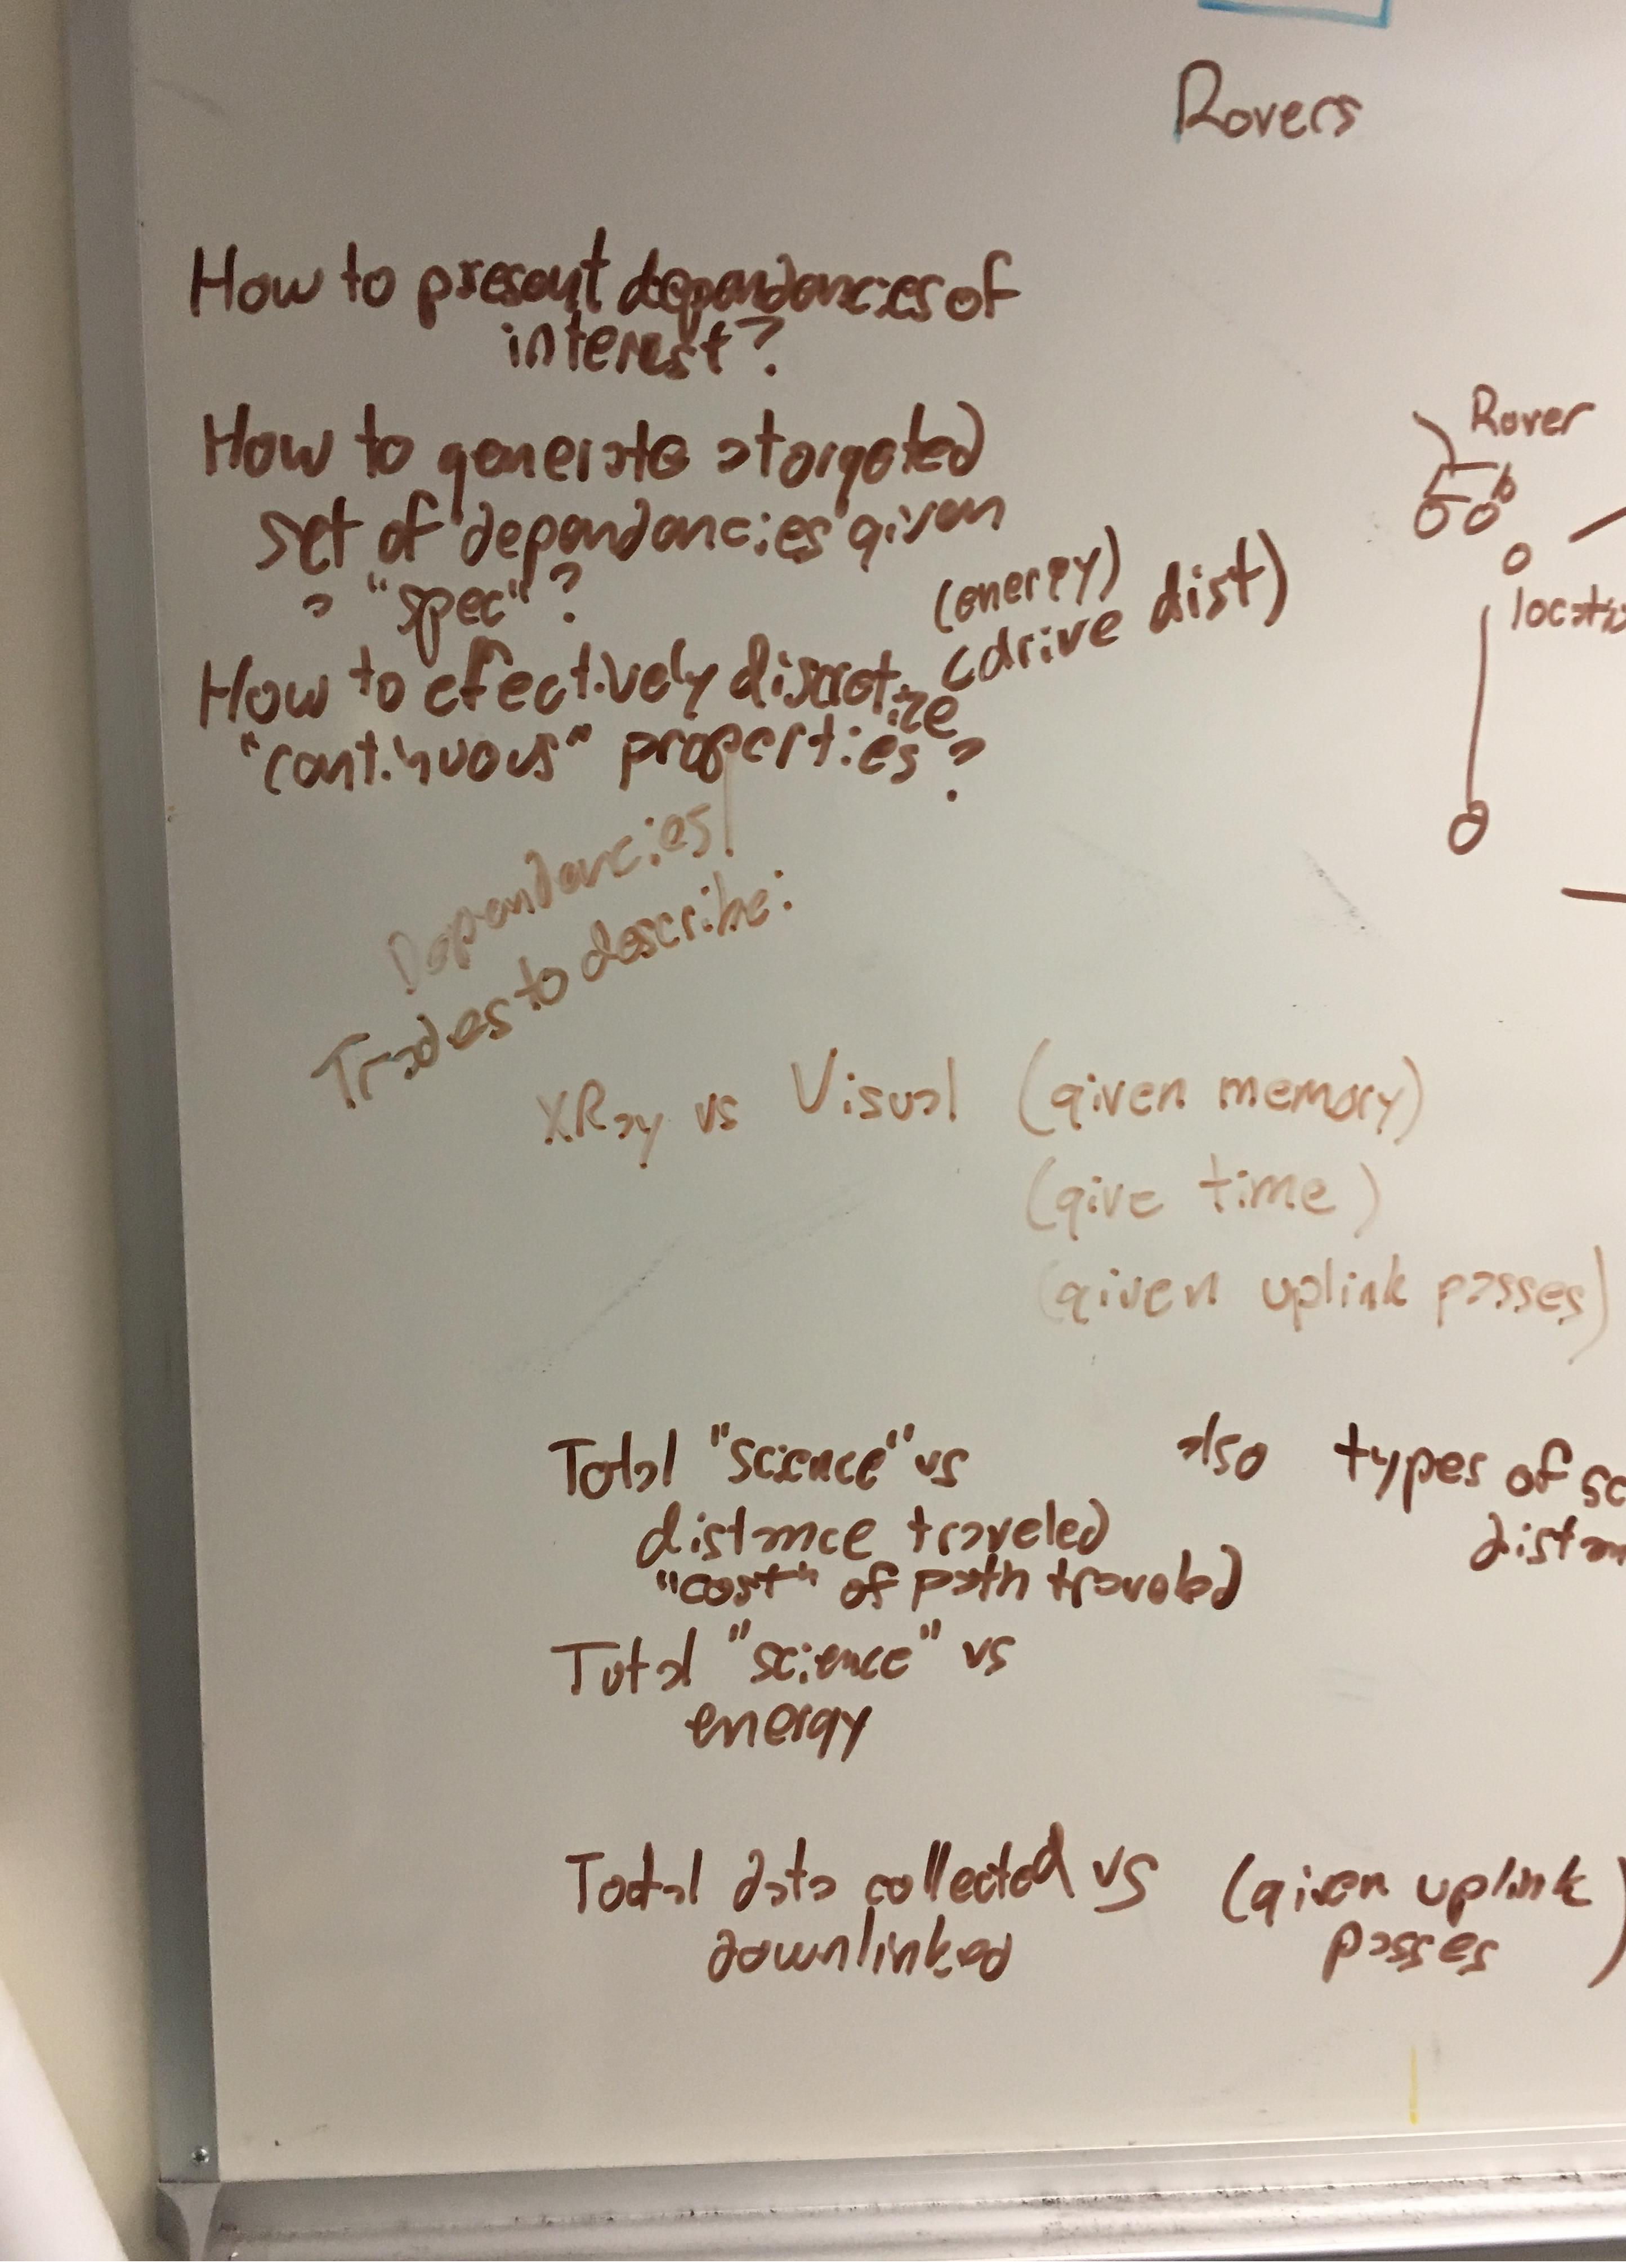
\includegraphics[height=8.0cm]{IMAGES/jeremy-whiteboard-rovers-1.JPG}
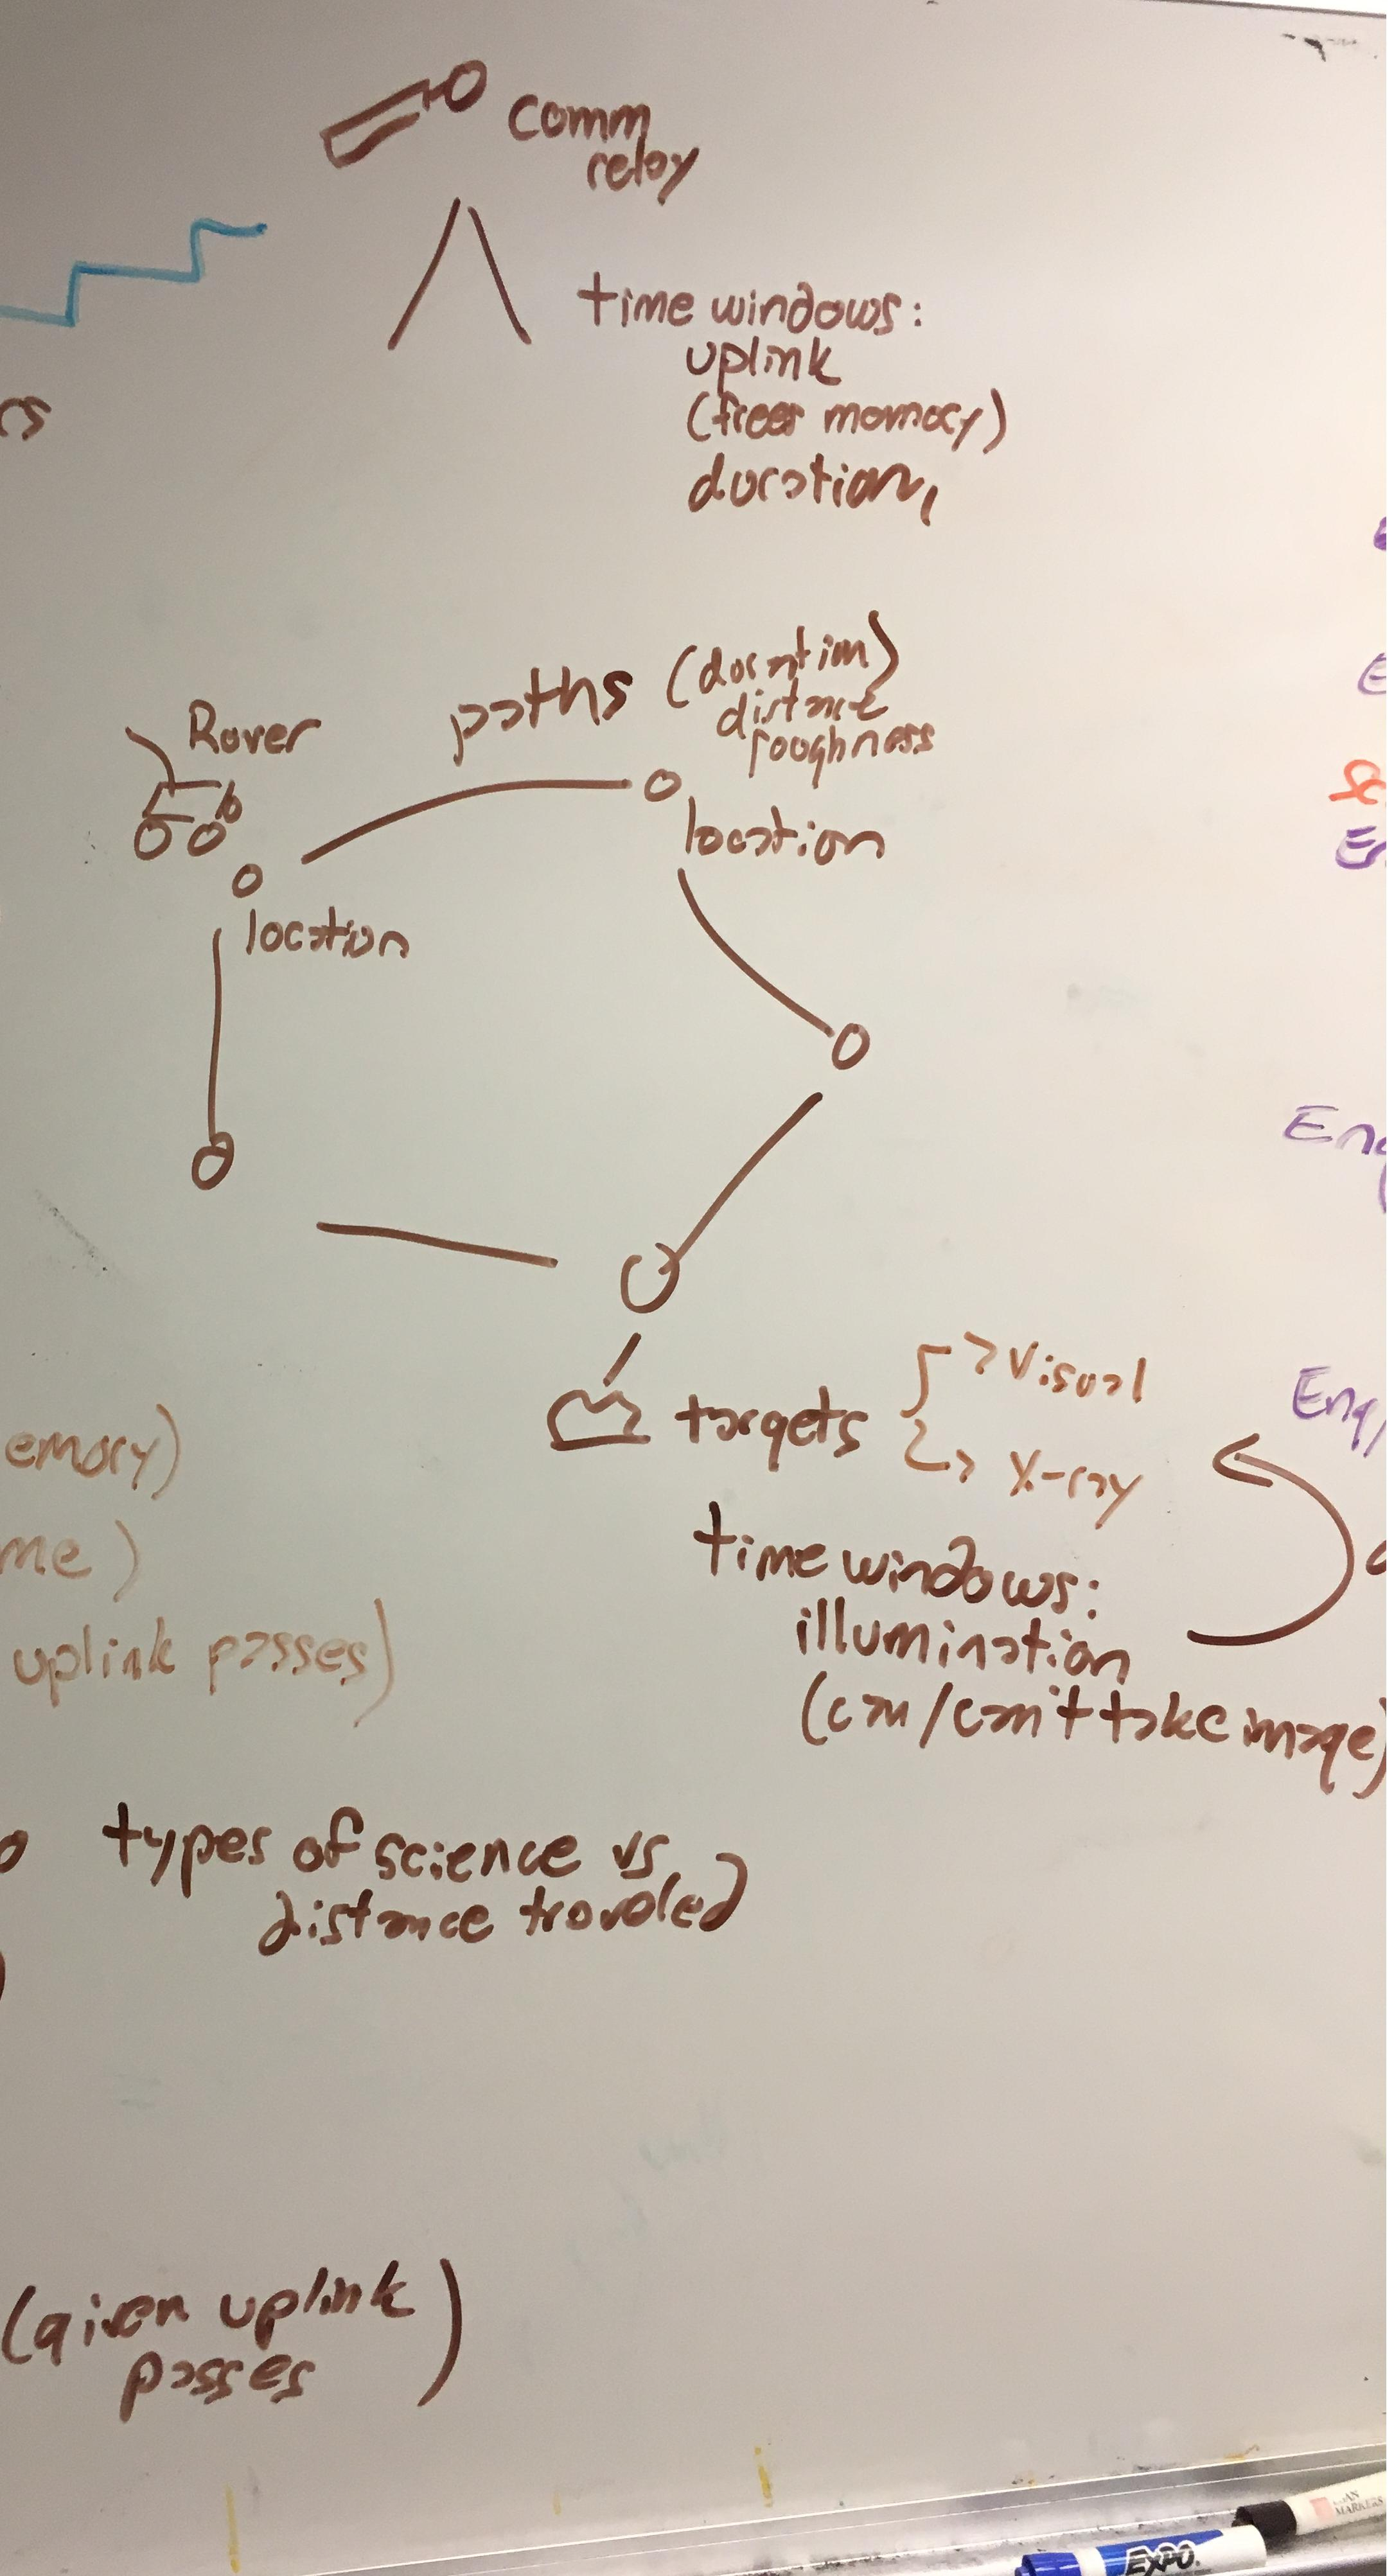
\includegraphics[height=8.0cm]{IMAGES/jeremy-whiteboard-rovers-2.JPG}
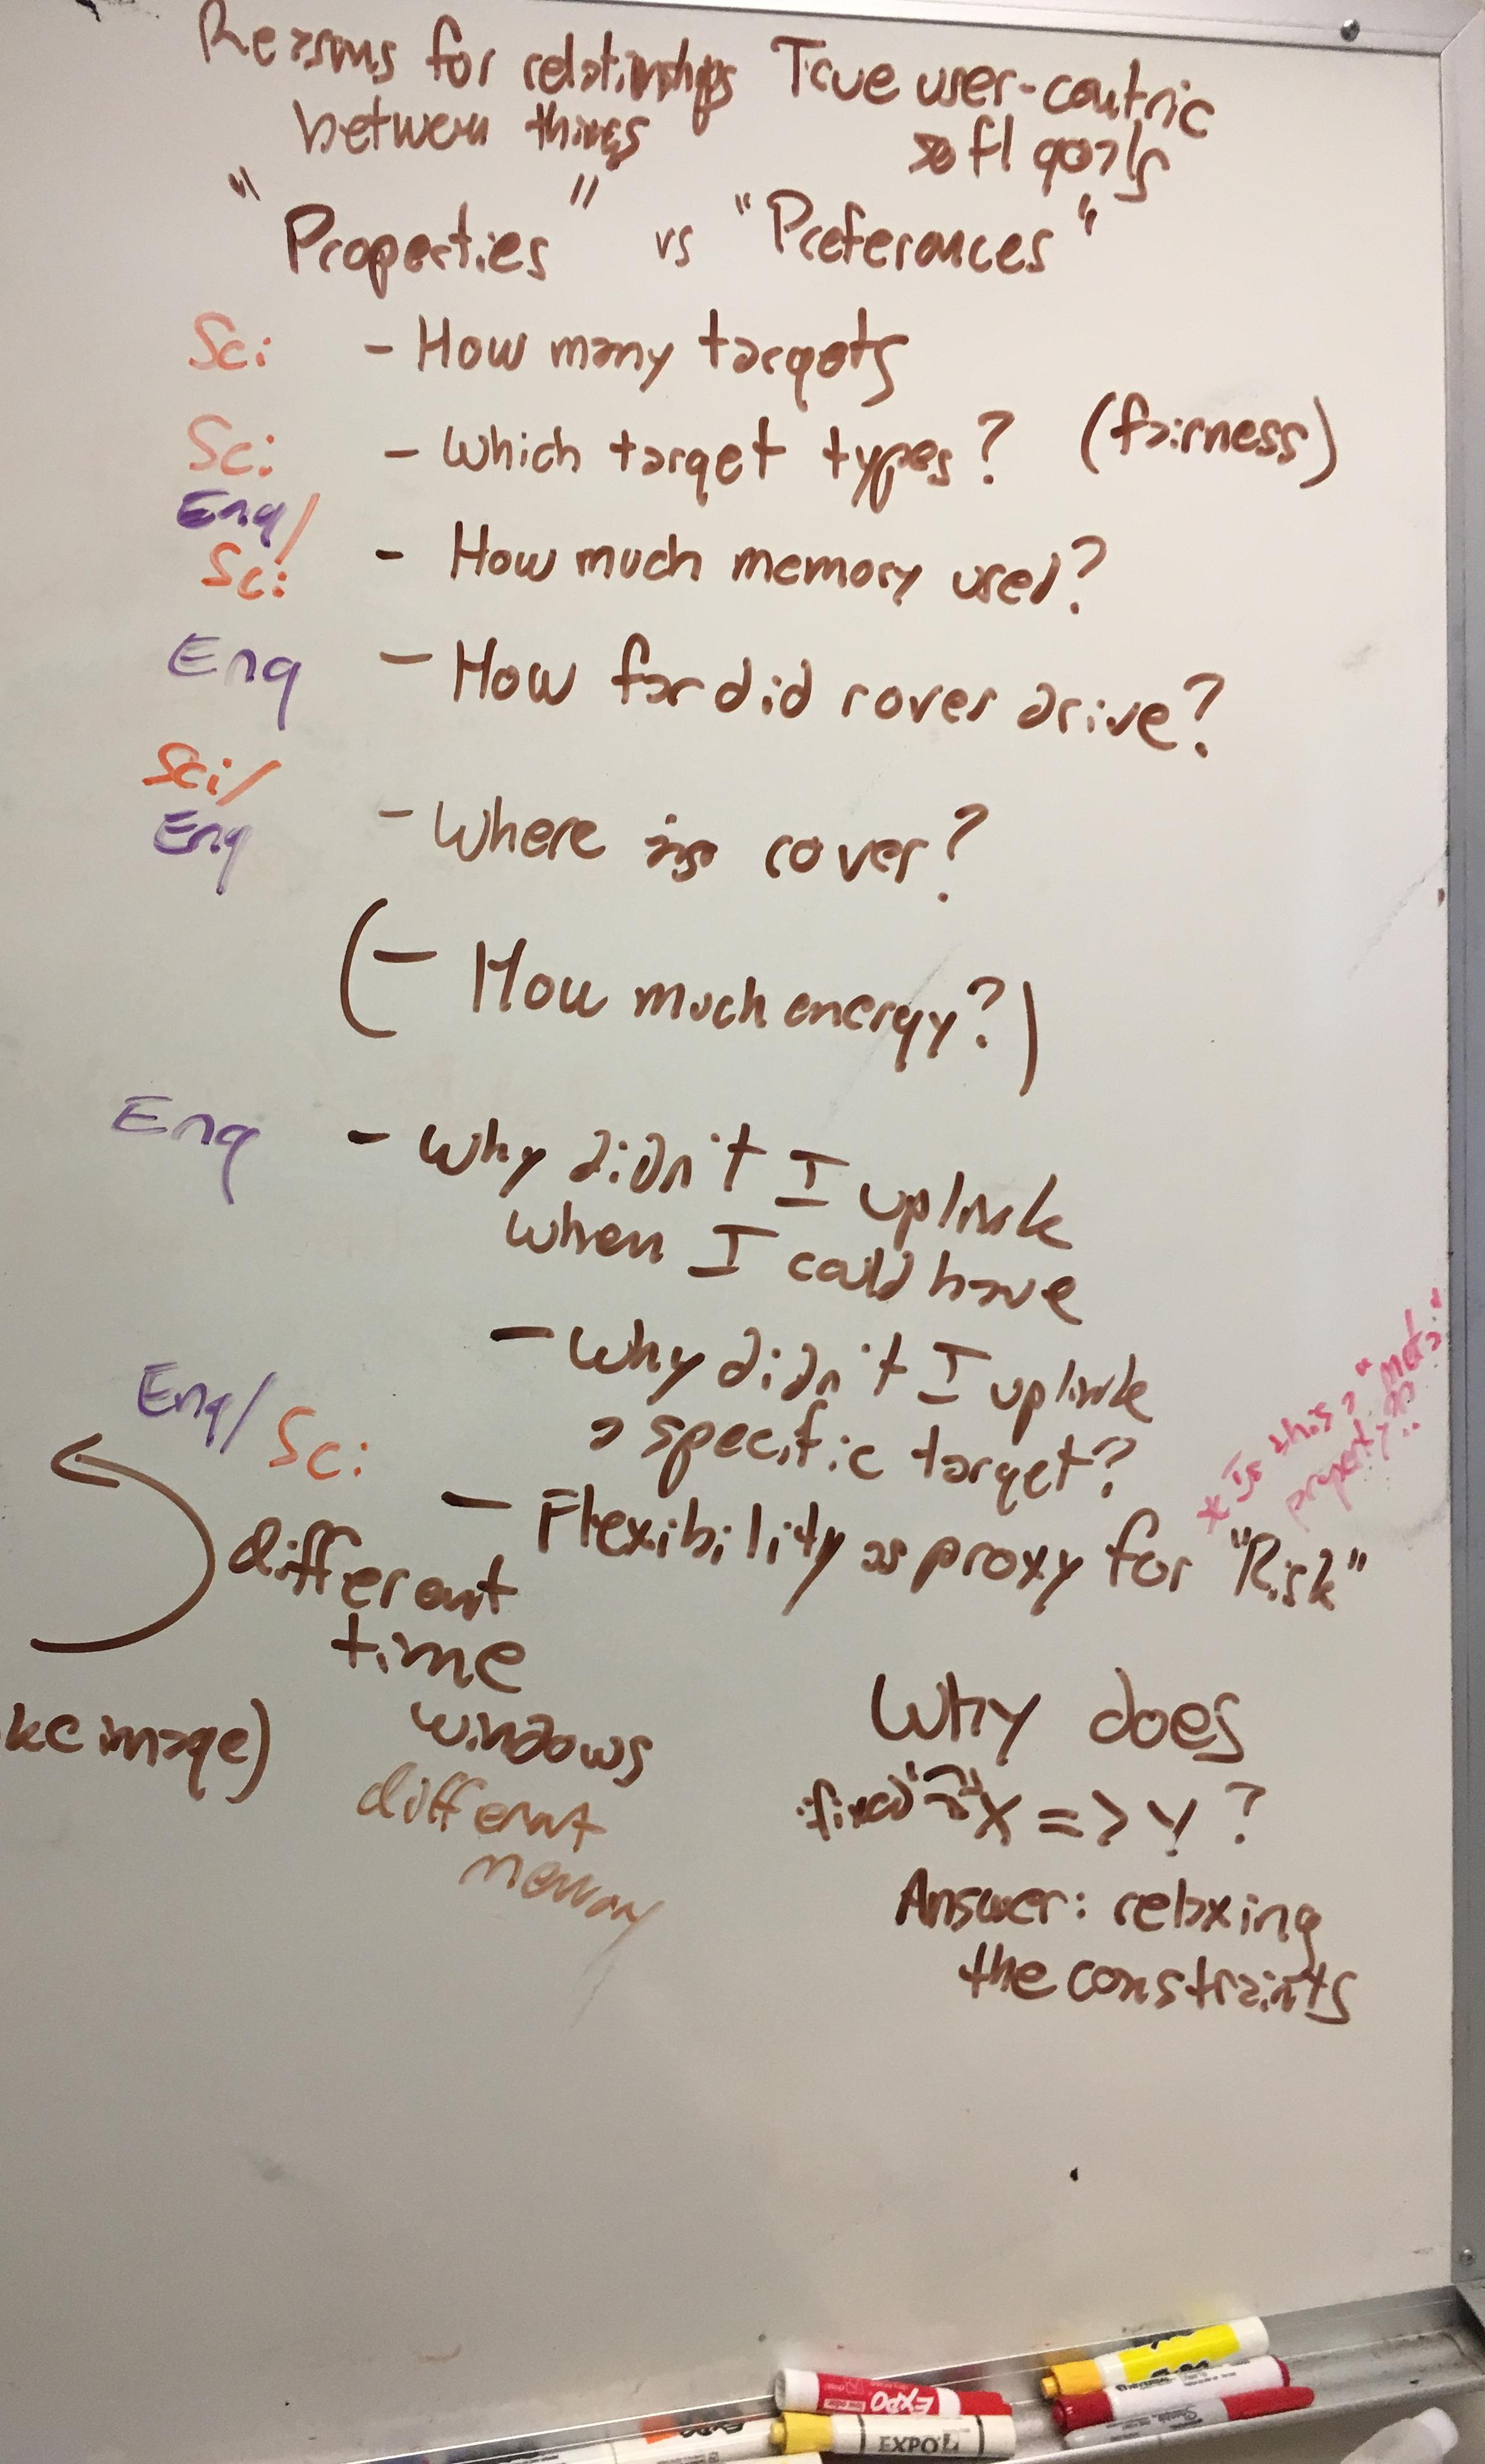
\includegraphics[height=8.0cm]{IMAGES/jeremy-whiteboard-rovers-3.JPG}


\subsection{Rovers model and properties}
\label{xpp-rovers:model}

Model: 
\begin{itemize}
\item rover
\item waypoints
\item paths: duration, cost for distance+roughness
\item targets: collection duration
\item target types (visual, x-ray, rock sample...)
\item feasability time windows for each target
\item amount of memory slots available (each target occupies one slot)
\item time windows for uplinking a given number of memory slots
\item energy level
\end{itemize}

Properties are grouped into ``dimensions'' meaningful to user, eg
different Boolean properties all discretizing amount of x-ray science
objectives achieved.


Property dimensions (that our objective is a function of):
\begin{itemize}
\item (scientists) fraction of targets collected by time point $T \geq
  X$?
\item (scientists) fraction of targets of type TT collected by time
  point $T \geq X$?
\item (scientists) distribution of fractions across types is fair?
\item (engineers) driving cost incurred by rover $\geq X$?
\item flexibility: slack in plan $\geq X$? 

  Serves as proxy for risk.

  (Or: how many concrete schedules does a given schedule permit?)
\item idle time in plan $\geq X$?

  When goals can't be achieved outside of specific time windows, idle
  time is often a consideration.  In cases like the rover domain where
  other 'non-goal-achieving' activities must be done (driving,
  uplinking), it may be hard to understand whether a plan looks good
  or bad from the perspective of idle-time. Intuitively, more science
  should translate to less idle time, but not always.  Furthermore,
  risk and idle time may be traded in interesting ways.

\end{itemize}


Property dimensions (that have causal influence on the above):
\begin{itemize}
\item \#memory slots available $\geq X$? [task property, not actionable]
\item maximal driving cost $\geq X$? [task property, actionable]
\item fraction of memory used at time point $T = X$?
\item rover at waypoint $X$?
\item target $X$ collected in time window $Y$?
\item uplink done in time window $Y$?
\item uplink done for target $X$ in time window $Y$?
\item amount of energy used $\geq X$?
\item amount of energy available $\geq X$? [model property! might be
  actionable]
\end{itemize}







\subsection{Rovers: expected dependencies and WHY/HOW questions}
\label{xpp-rovers:whyhow}


Example dependencies:
\begin{itemize}
\item A) fraction of targets of type x-ray collected at end of plan
  $\geq 40$\% $\Rightarrow$ fraction of targets of type visual
  collected at end of plan $< 20$\%.
\item B) \#memory slots available $< 7$ $\Rightarrow$ distribution of
  fractions across types is not fair.
\item C) uplink science objective A at time X $\Rightarrow$ don't
  achieve science objective B.
\end{itemize}

HOW questions: 
\begin{itemize}
\item eg A) how could this be improved? 

  \#memory slots available $\geq 20$ (not actionable); or maximal
  driving cost 132 (actionable)
\item 
\end{itemize}


WHY questions: 
\begin{itemize}
\item eg A) how could this be improved? 

  \#memory slots available $\geq 20$ (not actionable); or maximal
  driving cost 132 (actionable)

\item eg C) uplink science objective A at time X $\Rightarrow$ being
  at position P at time X $\Rightarrow$ missing time window Z for
  objective B $\Rightarrow$ having to use time window ZZ instead
  $\Rightarrow$ not enough energy
\end{itemize}









\subsection{Rovers: Concrete Model}
\label{xpp-rovers:concrete}

\joerg{to be designed based on PDDL/ongoing work IJCAI'19; extension
  to temporal PDDL if possible}


\section{XPP: Other Discussion Notes}
\label{xpp-discussion}





\subsection{Framework}

\begin{itemize}
\item Task properties? Boolean properties of task? Use these in our
  analyses just like plan properties?

  Totally relevant in planning with resources. Widen time windows a
  little bit in Rovers domain. 

  Seems crucial for HOW type of questions, with actionable changes
  becoming task properties.

  Formal handling: \plans\ changes as function of task properties. But
  straightforward when making enforced vs analyzed property sets
  explicit.

\item Discretization vs framework with numeric-valued plan properties

  Is there a way to get around need to discretize into Boolean
  properties? No ideas for this right now. 

  Discretization seems doable/Ok. Main issue is size, many props
  needed, combinatorial explostion of analysis. 

  $\Rightarrow$ How to effectively discretize, how to choose
  thresholds?

  Generalize from example instances?

  Instance-dependent: generate some example plans, glean relevant
  thresholds from there? (relats to user dialogue where user points
  out relevant/problematic properties of example plans).

\item Allow plan properties given as blackbox code supplied by user?

\item Flexibility: 

  Proxy for risk which is one source of preferences ie one
  soft/analyzed property to consider.

  Could think about making it a first-class citizen instead, but this
  would seem to basically just turn into an explicit user preference
  so it either relates to enforced plan properties or to a combination
  with user preferences.

\item Probability distribution over \plans, causality: Jeremy is
  unconvinced. The former conflicts with trade-off explicitation; the
  latter is explicitly captured in the planning state transition model
  if you're interested in it.

\item Only satisfiably plan props are of interest (in practice: filter
  unsat ones out first)

\end{itemize}




\subsection{Computation}

\begin{itemize}
\item Compute \plans\ once and then use it for everything?

\item \cool{BDDs for some of these computations? represent the set
  \plans?}

\item When using off the shelf planner to decide entailment: compile
  properties into derive predicates; could be a convenient tool /
  elegant write-up.

\item Approximation: compute \plans' subset or superset of \plans, test
  properties/dependencies against \plans'.

  Subset: counter-examples/falsify dependencies.

  Superset: sufficient criteria finding subset of valid dependencies.

  eg planning graph represents superset of \plans; mutex analysis is a
  special case of this very general framework.

\item Too many properties to analyze all dependencies, how to select
  relevant parts of PDO to be computed?

  Relates to user dialogue in interactive setting.

  Automatic property subset selection relates to property mining.

  Can we identify interesting dependencies, ie property pairs rather
  than properties, from example plans?

\end{itemize}





\subsection{XPP vs User Preferences}

\begin{itemize}
\item PDO relation to preference hierarchy? pref $p$ is stronger than
  $q$ is what it says; but importance to user is not there.

\item In iterative-planning application scenario, user preference
  incomplete is assumed: plan generator cannot generate unique most
  preferred solution with an up-front spec of preferences, else the
  iterative process would be useless.

\item Moving border between hard vs soft constraints as you go along,
  in the iterative process. makes sense both for iterative process and
  for computation.

\item There are three reasons for preference issues between user vs
  computer:

  1. different computational power, ie bounded rationality on part of
  user; eg ``why do we do task A after 4 pm?'' ie a dependency
  $\entails{\plans}{\true}{taskAafter4pm}$, or brilliant computer go
  move not understood by user.

  2. model differences (preconditions etc).

  3. optimization/preference function not fully specified up front.

  Here we don't address 2. (no explicit support for this; could be a
  future combination). 3. is naturally addressed in iterative planning
  process. 1. could be addressed, if we have the right plan properties
  to elucidate the ``causes'' behind a dependency. Interesting
  question for future work, see next subsec and
  Section~\ref{xpp:identify-causes} below.

\item Extension combination with user preferences?

  Combine/multiply/merge PDO with preference model over properties?

  Could eg deal point out inconsistent preferences

\item Ground prefs in the reality of feasible solutions, ie compute
  exact space of feasible preferred solutions. Not sure whether it
  makes sense computationally to first compute the entire PDO for this
  purpose though.

\item Or perhaps a more interactive approach where the PDO is
  navigated guided by user preferences, or vice versa user preferenes
  are navigated guided by the PDO?

\end{itemize}







\subsection{Generating Properties Relevant to User}

Mining as per proposal: start from seed set \props, compare example
plans with \prop\ vs $\neg \prop$, identify relevant differences based
on some sort of information about what's relevant to user, use
inductive learning to characterize these differenes with new plan
properties,

\begin{itemize}
\item Concrete example in oversubscription planning:

  User declared he cares about scientific objectives and energy
  consumption. Seed property objective A. In example plans with A we
  either don't have B, or don't have C, or consume a lot of energy. In
  example plans without A we sometimes have B and C and low energy
  consumption. Infer new property ``B and C and low energy''.

\item E.g. user worries about load balancing, not in \props; how to
  discover this?

  Proposal mining approach could work in principle, but load blanacing
  (variance) difficult to discover.

\item Make property mining interactive?

  Take inspiration from preference eicitation, in setting where
  analyzed properties are soft goals? Similarity is that we are
  looking for properties relevant to user preference; difference is
  that our goal is easier, we just need relevance, not a specification
  characterizing user preferences exactly.

  \cool{Example critiquing style:} Show a plan, user provides
  properties he likes/does not like, these props are included, and new
  plan is generated keeping the ``like'' while removing the ``don't
  like''?  This setup is very close to what
  \cite{fox:etal:ijcai-ws-17} proposed as a question answering method!
  That method here bcomes instead an input to our comprehensive
  analysis. 

\end{itemize}





\subsection{User Dialogues / Interfacing}

\begin{itemize}
\item Example critiquing cf above as interactive way to collect set of
  relevant properties.

  If generating an alternative plan takes too long, inform user ``I
  couldn't figure out how to do both $A$ and ``B''? Hm contains very
  little information. 

  \cool{More interesting: Suggest relaxations that would allow to do
    this! More fuel, more time, etc. $\Rightarrow$ relaxation
    operators in search space? relax completely first then accommodate
    as many constraints as possible?} Note that this relates closely
  to ``almost plans'' (to be used to find useful new plan properties
  for causal chain in WHY answer); it also relates to HOW answers, if
  the relaxations are actionable plan/task properties; also to excuses
  where basically the suggestion is an excuse. Main difference: online
  setting where instead of a complete analysis we are trying to be
  able to have suggestions in case the search for an alternate plan
  fails.

\item How to navigate the PDO:

  Select/modify subset of property dimensions considered. eg Rovers:
  xray vs visual given memory/time/uplink passed; total science vs
  distance traveled; total science vs energy; total data collected vs
  downlinked given uplink passes.

\end{itemize}










\subsection{Concrete Examples to look at}

\begin{itemize}
\item Classical planning blocksworld?

  Could be an option if we wanna go extreme on classical setting, and
  if the blocksworld stuff has phenomena inerestingf to talk a bout
  with plan properties. TBD.

\item Oversubscription rovers.

  Playground for NASA-style things but in simple basic setting.

  ``Classical'' version of oversubscription planning \ie\ classical
  planning but too many goals to achieve given amount of one consumed
  resource.

  Can go for temporal aspects where relevant, including Dan makes
  sense.

\item Crater reconstruction?

  Sun moves, rover has to take images of crater for 3D reconstruction,
  imaging depends on rover and sun location.

  Accurate formulation has complex continuous phenomena/consraints.

  Could go for a simple discrete temporal version in PDDL2.2 ie timed
  initial literals.

\item Mission planning?

  Over-subscription setting in online/mid-term scenario when something
  went wrong and not all objectives can be achieved
  anymore. Properties e.g. achieving an objective, using/not using a
  certain device, energy consumption, meeting/not meeting a deadline.

  The simplest version of this is if some task takes much longer than
  anticipated; as this happens, the ongoing decisions are: 1) keep
  going with this task (because it is important or urgent) and not do
  something else?  2) interrupt this task to do something even more
  important/urgent?  3) stop doing this task because it's not that
  important/urgent and it can be done later? Aside: some tasks take a
  very long time (days), and are interruptible.

  In this setting, the approach would at design-time address questions
  what implications a delay has, according to the model, on other
  tasks; at execution time the approach could serve as an iterative
  planning tool, enforcing delays if the consequences are ok.

  Note though: an inherent limitation here is that, the way the
  approach is formulated with plan properties being Boolean functions,
  that the set of plan properties considered would have to discretize
  the possible time points of task completion, ie the "delays" to
  consider would have to be a fixed set of constants.

\end{itemize}





\section{Application Characteristics/Models}

\subsection{Mission Planning}

\subsubsection{Time frame}

\begin{itemize}
\item Long-term (days/weeks/months): Mission control.

    Highly complex human planning. Individual teams for individual
    aspects. Highly interdependent problems (e.g. energy
    management/solar panels/trajectory planning), global constraint
    resolution in f2f meetings.
    
    Very difficult/impossible to model precisely. Lots of human
    judgement in what can/cannot be done, safety margins etc. No
    complete, global mathematical formulation (individual subsystems
    do have quite complex models, esp. power, attitude, thermal, life
    support), or even if so not reliable (considerable built-in margin
    to ensure safety).
    
    Some interest in automation (mostly for checking constraints, some
    for plan repair, less for 'de-novo' synthesizing full
    plans). Potential scalability issues (too many different spacehips
    to control) not on horizon. Main automation issue is different
    time frames see below.
    
\item Short-term immediate reaction (seconds): Emergency procedures.

    Possible emergencies that require immediate reaction essentially
    mapped out and trained for.

\item Mid-term (hours/1 day), with significant communication delays
  (one direction 2.5 min to Mars at close approach, or 22 min to Mars
  at furthest distance): Target for automation.

    Ultimate goal/desire from crews: "replace mission control" in
    answering of questions "what should we do right now?".
    
\end{itemize}


\subsubsection{Limitations of formal models}

\begin{itemize}
\item Safety margins

    Plan at abstract level, over- or under-approximation of safe
    behaviour.
    
    Can only ever be decision support/suggestion system, not fully
    automatic control.
    
    A lot of planning takes place to stay far away from anything that
    could develop into a safety-critical situation.
    
\item Critical tasks:

    The usual way time- and safety-criticality is discussed is in
    order of severity of tasks.  In decreasing order of severity:
    'loss of crew' (someone will be injured or die), 'loss of vehicle'
    (the spacecraft is going to be destroyed or damaged', 'loss of
    mission' (the actual mission objective can't be achieved but the
    spacecraft and crew will be fine', and then on to various
    'degradations', 'inefficiencies' (in time, resource use, etc.)
    
    The usual way of handling the worst safety critical tasks is that
    the crew simply drops everything and does what is needed, right
    away.  Planning as we envision it usually requires time to think.
    So situations in which replanning takes place will be somewhat
    less critical cases, or recovery after a major event when things
    are stabilized.

\item At design-time, use explainability as a tool towards refining
  the system/to eventually establish trust of mission control experts
  into the system.

    What kind of system refinement operations make sense here?

\end{itemize}


\subsubsection{Augment, not replace, mission control}

\begin{itemize}

\item Make the best of available channel.
    
\item Big question of human factors: How to communicate in an
  X-minutes delay setting? HCI research here. Simple measures like
  non-verbal communication/logs already seem to help a lot.
    
\item From planning perspective: mission control is a kind of oracle
  with delay (physical to/fro + estimated mission-control thinking
  time).
    
\item $\Rightarrow$ Interactive planning with delay? Interesting
  option. Need "interactive planning" framework first. Suggesting
  plans, accommodate plan feedback in next iteration? Iterative plan,
  question, explain framework as per Dan/Joerg AFOSR proposal,
  Section~\ref{xpp}? Human input in form of search guidance? Real-time
  aspects could also play a role here: make the best of the planning
  time available til the next round of feedback.
    
\item $\Rightarrow$ Simpler framework: incorporate feedback not into
  planning process itself, but into the plan. Temporal concurrent
  contingent planning where sensing actions model mission control
  feedback, with duration corresponding to delay?
    
\end{itemize}



\subsubsection{Mission Planning Models}

\begin{itemize}

\item Abstract models:

    May be useful to link explicitly, via predicate characterizations,
    to low-level state and behaviour (Jeremy prior work): detect
    inconsistencies, model refinement, etc.
 
\item Build on established procedures:

    Comprehensive coded responses to events etc.
    
    Highly complex, difficult to process for humans, case distinctions
    etc.
    
    Extreme end: "planning" would "just" instantiate standard
    procedures to current situation. But usually things are not this
    simple.  Procedures are very general conditional plans, so some
    amount of thought about how they apply is often needed.  Depending
    on circumstances, procedure duration and required resources change
    a lot.
    
    Therefore: planning = search over degrees of freedom within
    standard procedures?
    
\end{itemize}





\subsection{Robot Arm Planning}

\begin{itemize}

\item Temporal planning, but sequential. Currently PDDL2.1. Need
  "temporal flexibility" if things go wrong.

\item Partial contingency planning at design-time/offline:

    Action duration intervals, lower bound / average / upper bound
    
    Plan for average durations, insert contingencies "where most
    pertinent"
    
    Observation/sensing on conditions at time points
    
    "Pertinent" quantitatively in terms of degree of violation if
    deviations from average case
    
    RFF-style algorithm (see work by Teichteil-Koenigsbuch) to
    incrementally build partial policy, possibly by outer loop around
    standard temporal planner?
    
    Note: in sequential setting, time can be treated as a state
    variable
    
    Ex. early work by Dave Smith et al in a Europa context

\item Flexible dispatching/plan flexibility/robustness at
  execution-time/online:

    Suitable where degree of flexibility required is small enough to
    not require full-scale replanning
    
\item Disjunctive STNs with duration uncertainty: lighter-weight
  alternative to contingency planning, disjunctions model alternate
  ways to reach a node
    
\end{itemize}







\subsection{Levitating-Robot-with-Fans (better name?) Planning}

\begin{itemize}

\item Robot w/o legs, propelled by fans
   
\item If several robots, multi-agent path planning becomes relevant
  here? With uncertainty about the destinations of human agents?
  
\end{itemize}



\bibliographystyle{plain}
\bibliography{abbreviations,biblio,crossref}



\appendix

\section{XPP: AFOSR Project Abstract from project proposal}
\label{xpp-abstract}

In today's technological development, more and more technical systems
will take action decisions traditionally taken by humans. Where such
decisions directly affect economic value, or even human lives, it is
crucial for human users to be able to \textbf{check the decision
  rationales}. The ability to explain decisions suggested by a
computer system is, therefore, increasingly recognized as crucial to
the success and practicality of such systems.

The objective of the proposed project is to establish
\textbf{explanation facilities for AI Planning}, in terms of a
\textbf{Q\&A process}. Like other model-based control methodologies --
in difference to model-free control through ML methods -- AI Planning
lends itself naturally to explanation, as the reasoning process behind
the suggested decisions is explicit and can, in principle, be checked
by the human user. The difficulty then lies in actually making such
reasoning -- enumerating vast spaces of alternate decisions --
amenable to human users. Our central thesis is that this can be
naturally done in terms of \textbf{explaining the space of plans},
pointing out the most relevant \textbf{plan properties} and their
\textbf{dependencies}.

For example, in a robotics-planning application supporting underwater
vehicle control, given a plan of action suggested by the system, the
user may ask ``why not cover objective $x$?''; the answer could be
``covering $x$ would either require excessive time or energy, or
result in abandoning $y$ or $z$''.
Such an answer would be derived by considering the space of relevant
plan properties -- objectives covered, energy consumption, time -- and
examining their relative behavior within the space of plans. A user
question then translates into an enforced plan property $p$ (cover
objective $x$), and the answer is given in terms of the most relevant
(detrimental/non-trivial) plan properties $q$ entailed by $p$.

Given such an answer, the user may choose to ask a different question,
or -- if $p$ is desirable despite $q$ -- request an alternative plan
satisfying $p$. The Q\&A process then iterates until the user is
satisfied with the plan. Observe that, beyond explaining the system's
decisions to the user, such a process serves additional purposes:
\begin{itemize}
\item \textbf{The elaboration of user preferences}, often reflected
  imperfectly by the model, through an explanation-guided
  example-critiquing process.
\item \textbf{Interactive planning} via plan constraints iteratively
  imposed by the user, with in-depth support for understanding the
  implications of these constraints.
\end{itemize}
For example, previous work has proposed CyberSecurity applications
supporting network security penetration testing (pentesting) through
the identification of possible attack plans. The user preference here
pertains to the value of assets in the network, which is notoriously
hard to quantify; and interactive planning is key support for
elaborating a defense strategy. The Q\&A process then involves user
questions like ``what if I reconfigure host $x$ to remove the
vulnerability exploited here?'', and answers like ``the attack will
diverge to host $y$ instead, which would incur a high risk of being
detected''.

The proposed project will realize such a Q\&A analysis framework for
AI Planning. Our approach will be the inference of
\textbf{plan-property dependency networks (PDN)}. In such a network,
plan properties are arbitrary Boolean functions on plans;
and a property $p$ entails a property $q$ if all plans that satisfy
$p$ also satisfy $q$. For a more fine-grained analysis, we will infer
probabilistic forms of entailment, where the user preference is
modeled as a probability distribution over plans, capturing the
system's uncertainty about the actual user preference. The PDN then is
a \textbf{Bayesian network (BN) over plan properties}, compactly
representing dependencies weighted by plan likelihood.

Observe that, given a PDN, we can answer \emph{any} user question
about the underlying set of plan properties directly: by reading off
the entailments; and by standard BN reasoning techniques on
probabilistic dependencies. Thus we can \textbf{build the PDN
  offline}, performing the costly computations prior to the
\textbf{online user interaction}.

We will infer PDNs over a given set of properties through
\textbf{entailment checks}, formulated as planning-task unsolvability
proofs, where feasible. We will infer probabilistic dependencies
through \textbf{BN structure inference} from data, i.e., from
\textbf{sample plans} drawn from the desired probability distribution,
thus avoiding the -- practically infeasible -- enumeration of all
plans.
We will investigate the adequacy and feasibility of \textbf{causality}
analysis, i.e.\ the inference of cause-effect relations, in this
context. We will automate the \textbf{extraction of relevant plan
  properties} by generalizing from example plans through inductive
learning, identifying new composed properties that exhibit relevant
behavior (\eg, ``use excessive time or energy, or abandon $y$ or
$z$'').
We will develop user interfacing and user adaptation methods to
conveniently design, navigate, and modify the set of plan properties
considered.

We will realize this technology in \textbf{classical planning} first,
then investigate extensions to \textbf{temporal planning}, planning
under \textbf{limited resources}, and \textbf{oversubscription
  planning} (maximizing the reward from achieved goals subject to a
fixed resource budget). We will develop application demonstrators, on
top of a realistic ROS simulator for \textbf{underwater vehicle
  control}, and on top of realistic network data for
\textbf{pentesting}.



% joerg: moving target ...
%\section{XPP Framework (from IJCAI'19 paper draft)}
\label{xpp-framework}

We first introduce our approach making minimal assumptions on the
planning context and plan properties concerned. This serves to
identify the generic structure of the explainability problems we
target. That structure can then be instantiated with concrete planning
formalisms and plan-property languages of interest, as we will
exemplify in later sections.




\subsection{Planning Tasks and Plans}

We assume some formalism defining planning \defined{tasks} \task. We
do not need any assumptions about that formalism, except that it
defines a concept of \defined{plans} \plan, where that concept can
again be arbitrary (action sequence/schedule/partial order/etc). 

Our definitions are relative to a set of plans \plans\ of
interest. The canonical setup we have in mind is that where \plans\ is
\defined{implicit}, induced by \task\ as the set of \plan\ that
achieve a set of \defined{enforced} plan properties. But
\defined{explicit} \plans, given as a list of plans in the input, can
also be relevant if the user wants to focus the analysis on a
narrow/small subset of candidate plans. In either case, our framework
addresses dependencies between \defined{analyzed} plan properties
within \plans.
%
% Joerg: previous text here
%
%% Our definitions are relative to a set of plans \plans\ of interest:
%% the set of plan \emph{candidates} the human user is considering, and
%% whose property dependencies we should thus analyze. The canonical
%% setup we have in mind is that where \plans\ is \defined{implicit},
%% induced by \task\ as the set of \plan\ that achieve a set of
%% \defined{hard} goals/constraints (in general: \defined{plan
%%   properties}, see below) which the user is not willing to forego
%% under any circumstance. But \defined{explicit} \plans, given as a list
%% of plans in the input, can also be relevant if the user wants to focus
%% the analysis on a narrow/small subset of candidate plans. Whichever is
%% the case, the analysis considers dependencies between \defined{soft}
%% plan properties within \plans. These properties can be soft goals as
%% in oversubscription planning, but they can also be arbitrary
%% constraints characterizing the manner in which the hard plan
%% properties are achieved. For example, in classical planning,
%% \plans\ can simply be the set of (cost-optimal) plans achieving the
%% goal, where our analysis answers questions about the properties of
%% such plans.





\subsection{Plan Properties and Property Entailment}

Plan properties, in their most general form, are simply functions
mapping a task and plan to a Boolean value indicating whether or not
the property is satisfied:

\begin{definition}[Plan Property]
Denoting by \alltasks\ the set of all tasks and by \allplans\ the set
of all plans, a \emph{plan property} is a partial function $\prop :
\alltasks \times \allplans \mapsto \{\true, \false\}$. Given a task
\task\ and a set of plans \plans, we say that \prop\ is a plan
property defined on \task\ and \plans\ if its domain includes
$\{(\task,\plan) \mid \plan \in \plans\}$.
\end{definition}

Example plan properties are goal facts/goal formulas (true at end of
plan?), temporal plan trajectory constraints, constraints on subsets
of actions used/not used, deadlines, bounds on resource consumption,
etc. Canonically, $\prop$ is computable in time polynomial in the size
of its input.

We assume a set \props\ of plan properties (the analyzed ones) as part
of our input. In this context, a distinction not necessary for our
generic definitions, but important in practice, is that between
\defined{atomic} vs.\ \defined{composed} plan properties. The set
\propsatom\ of atomic properties is listed explicitly in the input,
whereas the composed properties \propscomp\ arise from a compact
specification how properties can be combined. For example, one may
define \propscomp\ to be propositional formulas over the atoms
\propsatom. Note that, given this, the set $\props = \propsatom \cup
\propscomp$ of plan properties whose dependencies are being analyzed
may be exponentially larger than the user input, and may even be
infinite.

As a concrete instance we will consider later on, the user may be
interested in a set $G$ of soft-goal facts, where for each $g \in G$
being or not being achieved by a plan $\plan \in \plans$ is an atomic
goal property. But the interesting dependencies may be, not across
individual $g$, but over conjunctions thereof (\eg\ if conjunctions,
but not typically singletons, exclude the possibility to achieve other
goals). The input to our analysis then is merely the set $G$, while
the analysis considers dependencies across all conjunctions over $G$.

The kind of dependency our framework focusses on is entailment over
plan properties, in the space of truth-value assignments induced by
the plan-candidate set \plans:

\begin{definition}[Entailment]
Let \task\ be a task and \plans\ a set of plans. Let \props\ be a set
of plan properties defined on \task\ and \plans.

Let $\plan \in \plans$. We identify \plan\ with the truth-value
assignment $\plan : \props \mapsto \{\true, \false\}$ where
$\plan(\prop) := \prop(\task,\plan)$. We identify \plans\ with the set
of such truth-value assignments. We say that
\plan\ \defined{satisfies} \prop, written $\plan \models \prop$, if
$\plan(\prop) = \true$. We denote by $\modelsof{\plans}{\prop} :=
\{\plan \mid \plan \in \plans, \plan \models \prop\}$ the models of
\prop. We say that \prop\ is \defined{satisfiable} in \plans\ if
$\modelsof{\plans}{\prop} \neq \emptyset$.

We say that \prop\ \defined{entails} \propq\ in \plans, written
$\entails{\plans}{\prop}{\propq}$, if $\modelsof{\plans}{\prop}
\subseteq \modelsof{\plans}{\propq}$.
%
We say that \prop\ and \propq\ are \defined{equivalent} in \plans,
written $\iff{\plans}{\prop}{\propq}$, if $\modelsof{\plans}{\prop} =
\modelsof{\plans}{\propq}$. The subset of \props\ equivalent with
\prop\ in \plans\ is written $\equiv{\plans}{\prop} := \{\propq \mid
\propq \in \props, \iff{\plans}{\prop}{\propq}\}$.
\end{definition}

This definition essentially just views plans $\plan \in \plans$ as
truth-value assignments in the obvious manner. Entailment and
equivalence over plan properties are then defined straightforwardly,
with \plans\ in the role traditionally taken by a knowledge base that
restricts the truth-value assignments under consideration. Recall that
formulas over plan properties can be encoded as individual composed
plan properties, so that defining entailment over individual plan
properties is enough to permit logical combinations thereof.

Importantly, the role of \plans\ as a knowledge base means that
entailment in \plans\ is more than standard entailment: the latter
implies the former, but not vice versa. As a simple example, say the
plan properties \props\ are propositional formulas $\phi$ over facts,
evaluated at the end of the plan. Then $\phi \Rightarrow \psi$ implies
that $\entails{\plans}{\phi}{\psi}$, simply because any (plan-end)
state that satisfies $\phi$ must satisfy $\psi$. But not vice versa:
\eg\ if facts $p, q$ are mutex in the task then
$\entails{\plans}{p}{\neg q}$. As a more motivating example, say the
plan properties are goals (like having scientific observations in
satellite planning) as well as resource constraints (like consuming at
most a given amount of energy). Then entailments of interest can take
the form $\entails{\plans}{p}{\neg q_1 \vee \neg q_2 \vee \neg q_3}$
saying that we cannot have $p$ without foregoing either of $q_1$ or
$q_2$ or $q_3$. Note that this is an entailment specific to \plans,
which may not hold in general (\eg\ if cheaper actions are available,
or if cheaper plans are admitted by removing some other hard
goals). It is precisely the identification of such specific
entailments -- specific to the space \plans\ of plans considered --
that motivates our approach.





\subsection{Plan-Space Explanation Problems}

Our plan-space explanation problems consist in identifying the
entailment relation on \props\ given the knowledge base \plans:

\begin{definition}[PDO and PDA]
Let \task\ be a task and \plans\ a set of plans. Let \props\ be a set
of plan properties defined on \task\ and \plans.

The \defined{plan-property dependency order (PDO)} for \plans\ and
\props\ is the partial order $\pdo{\plans}$ over the equivalence
classes $\equiv{\plans}{\prop}$, where $\equiv{\plans}{\prop}
\pdo{\plans} \equiv{\plans}{\propq}$ iff
$\entails{\plans}{\prop}{\propq}$.

A set $\pda{\plans} \subseteq \props$ is a \defined{plan-property
  dependency axiomatization (PDA)} for \plans\ and \props\ if, for
every minimal element $\equiv{\plans}{\prop}$ of $\pdo{\plans}$
restricted to \prop\ satisfiable in \plans, $\pda{\plans}$ contains
exactly one member of $\equiv{\plans}{\prop}$.
\end{definition}

% Joerg: not really needed, and potentially confusing in terms of what
% ``computing the PDO'' actually means -- how to represent the
% equivalence classes?
%
%% We refer by the \defined{PDO problem} to the computational problem of
%% computing the PDO given \task\ as well as a (compact) specification of
%% \props. Accordingly for the \defined{PDA problem}.

The PDO is a plan-space explanation in the sense of making explicit
how the plan properties of interest depend on each other -- saying
things like ``we cannot have $p$ without foregoing either of $q_1$ or
$q_2$ or $q_3$''. The PDO is exhaustive, and in that sense the ideal
plan-space explanation in principle. In practice though its size, \ie,
the number of equivalence classes, may be problematic. If one is
interested in atomic plan properties only, specified explicitly in the
user input, then \props\ and hence the PDO is small. If
\props\ includes composed properties though, then showing a PDA may be
more suitable.

A PDA captures the strongest properties, that together entail all
other properties given \plans\ -- and that, in this sense, form an
axiomatization for \plans. Unsatisfiable properties are not of
interest here as they trivially entail everything. For example, in
oversubscription planning, when plan properties are conjunctions of
soft goals, larger conjunctions entail smaller ones and a PDA
specifies the maximal solvable conjunctions.

%% We remark that the PDO is a meet-semilattice if $\props$ is closed
%% under conjunction, \ie, for every satisfiable $p, q \in \props$ there
%% is a satisfiable $r \in \props$ which is true if both $p$ and $q$ are
%% true. In this case, the PDA is a single plan property ... JOERG:
%% whatever. not gonna happen/who cares.
%
%% \joerg{reg lattices: $O$ is a ``meet-semilattice'' if $\Phi$ is closed
%%   under conjunction: in a lattice, every two elements need to have a
%%   common ancestor. in standard logic, entailment over formula
%%   equivalence classes is a lattice because for any $\phi$ and $\psi$
%%   $\phi \wedge \psi$ is a common ancestor; actually a bounded lattice,
%%   with a unique element that is an ancestor to (that implies)
%%   everything else. the same is true here if $\Phi$ is closed under
%%   conjunction (because if each of $\phi$ and $\psi$ is valid, then so
%%   is $\phi \wedge \psi$). In this case, the PDA is the unique common
%%   ancestor, which can basically be thought of as a conjunction of
%%   axioms. In lattice terminology, the unique common ancestor is called
%%   a ``least element'', ``minimum'', or ``bottom'' element; but I think
%%   none of these names makes much sense in our context so I would leave
%%   it at the above definition, maybe briefly remarking here that $O$ is
%%   a meet-semilattice if $\Phi$ is closed under conjunction.}

The PDO is finite if only atomic plan properties are considered,
simply as the number of truth-value assignments is. In the presence of
an infinite set of composed plan properties (such as propositional
formulas), the PDO may still be finite due to considering equivalence
classes. In particular, the latter is necessarily the case if the set
of plans \plans\ of interest is finite (as is the case \eg\ if the
action set is finite and plan size can be finitely bounded), because
then there is only a finite number of non-equivalent plan properties.

Regarding complexity, if \plans\ is implicitly given, then testing
plan-property satisfiability encompasses the plan existence problem
even for extremely simple plan properties (\eg, asking whether the
plan achieves some fact $p$). Similarly for plan-property entailments
$\entails{\plans}{\prop}{\propq}$, proving which corresponds to
proving a planning task unsolvable (there exists no plan that
satisfies \prop\ but not \propq). Tractable cases are limited to
explicitly given \plans, and planning fragments where \plans\ -- the
set of all plans -- can be generated in polynomial time. This is
exacerbated by the potentially exponential size of the PDO, and the
PDA, for composed plan properties. Certainly, both the PDO and PDA
problems should ideally be solved offline, prior to interaction with a
user. As our experimental results show, however, in a variety of
benchmarks, computing a PDA has similar scalability as optimal
planning, and the size of a PDA is reasonably small for human
inspection.


% Joerg: a fully formal frame here would need to talk about
% compilations, also of planning tasks ... overkill, instead formulate
% what's needed in the concrete instances here when we get there.
%
%% A property we will rely on in the following sections is that sometimes
%% a PDA for a plan-property set $\props^B$ can be easily obtained from
%% that for a plan-property set $\props^A$:
%
%% \begin{definition}[PDA Derivability]
%% Let $\props^A$ and $\props^B$ be sets of plan properties. We say that
%% a PDA for $\props^B$ is \defined{polynomially derivable} from that for
%% $\props^A$ if there exists an algorithm that runs in time polynomial
%% in the size of its input and that, for any task \task\ on which all
%% $\prop \in \props^A \cup \props^B$ are defined, transforms a PDA for
%% $\props^A$ into one for $\props^B$.
%% \end{definition}





\section{Chronological Meeting/Discussion Notes}

\begin{itemize}
\item Dec 3: Jeremy/Minh/Joerg: 

    Mission Planning Application Characteristics, Mission Planning Models

\item Dec 5: Jeremy: 

    Feedback on writeup
    
\item Dec 6: Jeremy/Rob/Joerg: 

    Robot arm planning, plan flexibility, contingency planning
        
\item Dec 11: Jeremy/Dave/J/Minh/Joerg: 

    XPP discussion and future directions

\item Dec 14: Jeremy:

  Framework discussion, Rovers example

\item Dec 17: Jeremy:

  Framework discussion, Rovers example

\item Dec 18: Jeremy:

  Finding properties, navigating the PDO, Rovers example

\item Dec 19: Dave:

  User dialogues, relevance filter on PDO

\end{itemize}




\end{document}
